\documentclass{jsarticle}
\usepackage{amsmath}
\usepackage{amssymb}
\usepackage{ascmac}
\usepackage{bm}
\usepackage{graphicx}

\flushbottom
\sloppy

\setlength{\paperwidth}{210mm}
\setlength{\paperheight}{297mm}
\setlength{\voffset}{0mm}
\setlength{\textwidth}{\paperwidth}
\addtolength{\textwidth}{-30mm}
\setlength{\textheight}{\paperheight}
\addtolength{\textheight}{-50mm}
\setlength{\topmargin}{-1in}
\addtolength{\topmargin}{20mm}
\setlength{\headheight}{0mm}
\setlength{\headsep}{0mm}
\setlength{\footskip}{20mm}
\setlength{\oddsidemargin}{-1in}
\addtolength{\oddsidemargin}{15mm}
\setlength{\columnsep}{7mm}

\title{\Large {\bf クラスタリングとGMM ― 複合システムモデルを同定する二つのアプローチ}}
\author{杉原知道}

\begin{document}
%\thispagestyle{empty}

\maketitle

%%%%%%%%%%%%%%%%%%%%%%%%%%%%%%%%%%%%%%%%%%%%%%%%%%%%%%%%%%%%%%%%%%%%%%
\section{やりたいこと}

ある未知の代数的システム(与えられた代数方程式を満たす全ての変数の集合)
$\mathcal{S}=\{\bm{x}|\bm{f}(\bm{x})=\bm{0}\}$($\bm{x}$はシステム変数)
から
標本群$\mathcal{X}=\{\bm{x}_{i}\}$($i=1,\cdots,N$)が観測によって得られたとして,
これらからシステムのモデル$\hat{\mathcal{S}}=\{\bm{x}|\hat{\bm{f}}(\bm{x};\bm{\theta})=\bm{0}\}$
($\bm{\theta}$はシステムパラメータ)を同定することを考えます.
具体的には,$\bm{\theta}$を最小二乗法で求める問題になります.
\begin{align*}
\bm{\theta}=\mathop{\mathrm{arg~min}}_{\bm{\theta}}
\left\{
E(\bm{\theta};\mathcal{X})=\frac{1}{2}\sum_{i=1}^{N}\bm{e}_{i}^{\mathrm{T}}\bm{e}_{i}
\right\}
\end{align*}
ただし,$\bm{e}_{i}\overset{\mathrm{def}}{=}\hat{\bm{f}}(\bm{x}_{i};\bm{\theta})$です.
$E(\bm{\theta};\mathcal{X})$が
「$\mathcal{X}$が与えられた下での$\bm{\theta}$の関数」であることに注意して下さい.
$\hat{\bm{f}}(\bm{x};\bm{\theta})$が$\bm{\theta}$に対し微分可能
かつ$E(\bm{\theta};\mathcal{X})$が下に凸であれば,
次の方程式を解くことにより$\bm{\theta}$が得られます.
\begin{align*}
\left(\frac{\partial E}{\partial\bm{\theta}}\right)^{\mathrm{T}}=\bm{0}
\quad\Leftrightarrow\quad
\sum_{i=1}^{N}\left(\frac{\partial\hat{\bm{f}}(\bm{x}_{i};\bm{\theta})}{\partial\bm{\theta}}\right)^{\mathrm{T}}\hat{\bm{f}}(\bm{x}_{i};\bm{\theta})=\bm{0}
\end{align*}
以下,
$\bm{x}$,$\bm{f}(\bm{x})$,$\bm{\theta}$の次元がそれぞれ$n$,$m$,$p$であるとします.

\begin{quote}
\noindent{\bf 【例1】}
$\hat{\bm{f}}(\bm{x};\bm{\theta})=\bm{x}-\bm{\theta}$($p=m=n$)の場合,
\begin{align*}
\left(\frac{\partial E}{\partial\bm{\theta}}\right)^{\mathrm{T}}=\bm{0}
\quad\Leftrightarrow\quad
\sum_{i=1}^{N}(\bm{x}_{i}-\bm{\theta})=\bm{0}
\quad\Leftrightarrow\quad
\bm{\theta}=\frac{1}{N}\sum_{i=1}^{N}\bm{x}_{i}
\end{align*}
つまり,$\bm{\theta}$は$\bm{x}_{i}$の平均です.
\end{quote}
\begin{quote}
\noindent{\bf 【例2】}
$\hat{\bm{f}}(\bm{x};\bm{\theta})=\bm{\theta}^{\mathrm{T}}\bm{x}-1$($p=n, m=1$)の場合,
\begin{align*}
\left(\frac{\partial E}{\partial\bm{\theta}}\right)^{\mathrm{T}}=\bm{0}
\quad\Leftrightarrow\quad
\sum_{i=1}^{N}\bm{x}_{i}(\bm{x}_{i}^{\mathrm{T}}\bm{\theta}-1)=\bm{0}
\quad\Leftrightarrow\quad
\bm{\theta}=\left(\sum_{i=1}^{N}\bm{x}_{i}\bm{x}_{i}^{\mathrm{T}}\right)^{-1}\sum_{i=1}^{N}\bm{x}_{i}
\end{align*}
ちなみにこの例の$\mathcal{S}$は,
$\bm{\theta}$を法線方向ベクトルとする平面上の点群により構成されるシステムを表しています.
右辺の計算は$\sum_{i=1}^{N}\bm{x}_{i}\bm{x}_{i}^{\mathrm{T}}$が正則な場合にのみ可能で,
このため少なくとも$N\geq p$でなければなりません.
\end{quote}

次に,システム全体が$K$個の相異なる部分システム$\mathcal{S}_{k}$($k=1,\cdots,K$)の直和
$\mathcal{S}=\mathcal{S}_{1}+\cdots+\mathcal{S}_{K}$である場合を考えましょう.
$\mathcal{S}_{k}$($k=1,\cdots,K$)を,
パラメータ$\bm{\theta}_{k}$を用いて
$\hat{\mathcal{S}}_{k}=\{\bm{x}|\hat{\bm{f}}_{k}(\bm{x};\bm{\theta}_{k})=\bm{0}\}$とモデル化します
($\bm{\theta}_{k}$の要素数は全て$p$であるとします).
$\mathcal{X}$から全ての$\bm{\theta}_{k}$を同定するためには,
先にそれぞれの標本がどの部分システムに所属するか推定しなければなりません.
しかしそれぞれの標本がどの部分システムに所属するか正しく推定するためには,
全ての$\bm{\theta}_{k}$が同定されていなければなりません.
この典型的なchicken-and-egg問題をどのように解くかが本記事の本題です.


%%%%%%%%%%%%%%%%%%%%%%%%%%%%%%%%%%%%%%%%%%%%%%%%%%%%%%%%%%%%%%%%%%%%%%
\section{クラスタリング($K$-means法)によるモデル同定}

\subsection{$K$-means法}

{\bf $K$-means法}\cite{bib:macqueen1967,bib:duda1973}は,
全標本がそれぞれどの部分システムに所属するか,次のアルゴリズムで陽に推定する方法です.
\begin{screen}
\begin{enumerate}
\setlength{\itemsep}{-.2\baselineskip}
\item{観測された全標本を$K$個のグループに適当に分割し,
各部分システム$\mathcal{S}_{k}$($k=1,\cdots,K$)に所属する標本群(クラスタ)の初期候補$\mathcal{C}_{k}$($k=1,\cdots,K$)とする.}
\item{各$\mathcal{C}_{k}$に所属する標本群を用いて$\bm{\theta}_{k}$をそれぞれ同定する.}
\item{各$\bm{x}_{i}$に対し$\bm{e}_{ik}=\hat{\bm{f}}_{k}(\bm{x}_{i};\bm{\theta}_{k})$($k=1,\cdots,K$)を求め,
最も小さい$\|\bm{e}_{ik}\|$を与える$\mathcal{C}_{k}$にその標本を改めて所属させる.
}
\item{3において所属変更された標本が無ければ終了.さもなければ2に戻る.}
\end{enumerate}
\end{screen}
ただし,オリジナルの$K$-means法における平均および平均から各標本までの距離計算を,
それぞれ$\bm{\theta}_{k}$の同定と$\bm{e}_{ik}$の計算に読み替えています.
可視化すればアルゴリズムのプロセスは一目瞭然なのですが,
横着してそれは他記事に委ねます.

\subsection{良い結果を得るための初期クラスタ候補配置}

$K$-means法の結果は初期クラスタ候補の配置に依存します.
良い結果 --- クラスタ間の分離度が高い結果 --- を得るためには,
初期クラスタ候補をお互いになるべく離れた所に配置すべきです.
このような発想に基づく方法として,
{\bf KKZ法}\cite{bib:katsavounidis1994}と呼ばれる次の手順が知られています.
\begin{screen}
\begin{enumerate}
\setlength{\itemsep}{-.2\baselineskip}
\item{$\mathcal{X}$の元のうち,互いに最も離れた二つを
$\bm{x}^{*}_{1}$,$\bm{x}^{*}_{2}$とする.
\begin{align*}
(\bm{x}^{*}_{1},\bm{x}^{*}_{2})=\mathop{\mathrm{arg~max}}_{(\bm{x},\bm{y})}\left\{d(\bm{x},\bm{y})
\left|
\forall\bm{x}\in\mathcal{X},
\forall\bm{y}\in\mathcal{X},
\bm{x}\neq\bm{y}
\right.
\right\},\quad
\mathcal{C}_{1}=\left\{\bm{x}^{*}_{1}\right\},\quad
\mathcal{C}_{2}=\left\{\bm{x}^{*}_{2}\right\}
\end{align*}
ただし$d(\bm{x},\bm{y})$は変数が所属する空間のメトリック
(ユークリッド空間ならば$d(\bm{x},\bm{y})\equiv\left\|\bm{x}-\bm{y}\right\|$).
}
\item{$k=3$とする.}
\item{$\mathcal{X}$から$\bm{x}^{*}_{1},\cdots,\bm{x}^{*}_{k-1}$を除いた
$\mathcal{X}_{k}\overset{\mathrm{def}}{=}\mathcal{X}\setminus\left\{\bm{x}^{*}_{1},\cdots,\bm{x}^{*}_{k-1}\right\}$
の元の中から,
$\bm{x}^{*}_{1},\cdots,\bm{x}^{*}_{k-1}$のうち
最小距離を与える点への距離が最大となるものを$\bm{x}^{*}_{k}$とする.
\begin{align*}
\bm{x}^{*}_{k}=\mathop{\mathrm{arg~max}}_{\bm{x}}\left\{
\left.
\min_{j=1,\cdots,k-1}d(\bm{x},\bm{x}^{*}_{j})
\right|
\forall\bm{x}\in\mathcal{X}_{k}
\right\},\quad
\mathcal{C}_{k}=\left\{\bm{x}^{*}_{k}\right\}
\end{align*}
}
\item{$k<K$ならば,$k\leftarrow k+1$として3へ戻る.}
\item{
残りの全ての標本
$\forall\bm{x}_{i}\in\mathcal{X}_{K+1}=\mathcal{X}\setminus\left\{\bm{x}^{*}_{1},\cdots,\bm{x}^{*}_{K}\right\}$
を,
$\bm{x}^{*}_{1},\cdots,\bm{x}^{*}_{K}$のうち最も近いものと同じグループに所属させ,
初期クラスタ候補$\mathcal{C}_{k}$($k=1,\cdots,K$)を確定する.
\begin{align*}
k=\mathop{\mathrm{arg~min}}_{k=1,\cdots,K}d(\bm{x}_{i},\bm{x}^{*}_{k})
\\
\mathcal{C}_{k}\leftarrow\mathcal{C}_{k}\cup\left\{\bm{x}_{i}\right\}
\end{align*}
}
\end{enumerate}
\end{screen}
なお,KKZというのは上記引用文献の著者3人の頭文字をつなげたものです.

この方法は,観測された標本の中に外れ点(アウトライア)が混ざっている場合に,
それに引っ張られて結果が悪化するという弱点があります.
そこで,
上記手順のうち3を
\begin{screen}
\begin{enumerate}
\setcounter{enumi}{2}
\setlength{\itemsep}{-.2\baselineskip}
\item{$\mathcal{X}$から$\bm{x}^{*}_{1},\cdots,\bm{x}^{*}_{k-1}$を除いた
$\mathcal{X}_{k}\overset{\mathrm{def}}{=}\mathcal{X}\setminus\left\{\bm{x}^{*}_{1},\cdots,\bm{x}^{*}_{k-1}\right\}$
の元それぞれについて,$d_{i}$を次式で求める.
\begin{align*}
d_{i}=\min_{j=1,\cdots,k-1}d(\bm{x},\bm{x}^{*}_{j})
\end{align*}
$\mathcal{X}_{k}$の元から$\bm{x}_{i}$が選ばれる確率を$\displaystyle\frac{d_{i}}{\sum_{j=1}^{N-k+1}d_{j}}$として,
乱数的に一つ選択し$\bm{x}^{*}_{k}$とする.
}
\end{enumerate}
\end{screen}
と置き換えることで,
確率的に外れ点の影響から逃れる方法も提案されています.
これは{\bf $K$-means$++$法}\cite{bib:arthur2007}と呼ばれます.
いずれにしても確率的に外れ点を選択してしまう可能性は免れないので,
$K$-means法を何度か試行して最も良い結果を採択する,
というやり方が実用上は必須です.

結果の良し悪しの評価方法としては,
次に説明する{\bf シルエット分析}\cite{bib:rousseeuw1987cam}がよく知られています.
まず,全標本に対して次の$s_{i}$(シルエット)を計算します.
\begin{align*}
s_{i}=\frac{b_{i}-a_{i}}{\mathrm{max}\left\{a_{i},b_{i}\right\}}
\end{align*}
ただし,
\begin{align*}
a_{i}=D(\bm{x}_{i};\mathcal{C}_{\left\{\bm{x}_{i}\right\}})
\\
b_{i}=\min_{\mathcal{C}\neq\mathcal{C}_{\left\{\bm{x}_{i}\right\}}}D(\bm{x}_{i};\mathcal{C})
\\
D(\bm{x};\mathcal{C})\overset{\mathrm{def}}{=}
\sum_{\bm{x}_{j}\in\mathcal{C}}
\frac{d(\bm{x}_{j},\bm{x})}{\left|\mathcal{C}\right|}
\end{align*}
で,
$\mathcal{C}_{\left\{\bm{x}_{i}\right\}}$は$\bm{x}_{i}$の所属するクラスタ,
$\left|\mathcal{C}\right|$はクラスタ$\mathcal{C}$の要素数を表します.
原典では$a_{i}$の計算において$\bm{x}_{i}$自身を$\mathcal{C}_{\left\{\bm{x}_{i}\right\}}$から除いているのですが,
その場合は$\mathcal{C}_{\left\{\bm{x}_{i}\right\}}=\left\{\bm{x}_{i}\right\}$となったときに例外処理が必要となるので,
本記事では敢えてそのようなことをしない定義を採用します.

$s_{i}$は$-1\sim 1$の値をとり得ます.
定性的には,
クラスタ$\mathcal{C}_{\left\{\bm{x}_{i}\right\}}$の凝集度が高いと$a_{i}$が小さく,
クラスタ間の分離度が高いと$b_{i}$が大きくなるので,
$\bm{x}_{i}$がうまくクラスタリングされていれば$s_{i}$は$1$に近く,
そうでなければ$-1$に近くなります.
平均シルエット$\bar{s}$
\begin{align*}
\bar{s}=\frac{1}{N}\sum_{i}^{N}s_{i}
\end{align*}
が大きいほど,良好な結果が得られていると言えます.


\subsection{クラスタ数$K$はどのように選ぶ?}

$K$が未知の場合は,
幾つか異なる$K$について$\hat{\mathcal{S}}$を得た後,
最も良い結果を与えた$K$を選択するのが良いでしょう.
この評価にもシルエット分析が応用できます\cite{bib:deAmorim2015is}.
前節で説明した事柄から単純に考えれば,
平均シルエット$\bar{s}$が最大となる$K$を選べば良いように思えますが,
$K$を大きくして外れ点を全て独立したクラスタとすることで$\bar{s}$を大きくすることも,理論上可能です.
したがって,各クラスタの持つ標本数に大きく隔たりが無いかどうかも考慮に入れなければなりません.
実用上は,
全てのクラスタの最大シルエット$\max_{\bm{x}_{i}\in\mathcal{C}_{k}}s_{i}$が平均シルエット$\bar{s}$より大きいものの中で,
最小クラスタ数と最大クラスタ数の比
$\displaystyle\frac{\max_{k=1,\cdots,K}\left|\mathcal{C}_{k}\right|}{\min_{k=1,\cdots,K}\left|\mathcal{C}_{k}\right|}$
が最小となるような$K$を採用する,という規範が採用されます.

\subsection{$X$-means法 --- クラスタを再帰的に自動分割するアルゴリズム}

評価値に基づいて再帰的にクラスタを自動分割していく{\bf $X$-means法}\cite{bib:pelleg2000}という方法も提案されています.
アルゴリズムは次の通りです(オリジナルのものを少々変更しています).
\begin{screen}
\begin{enumerate}
\setlength{\itemsep}{-.2\baselineskip}
\item{まず$K=1$と仮定し,全標本から$\hat{\mathcal{S}}$を同定する.}
\item{モデルの同定精度を評価する(同定精度に対し単調減少な)指標値$I(\hat{\mathcal{S}})$を計算する.}
\item{次に,
システムを2つのサブシステムの直和$\hat{\mathcal{S}}^{\prime}=\hat{\mathcal{S}}_{\mathrm{A}}+\hat{\mathcal{S}}_{\mathrm{B}}$としてモデル化し,
同定する.}
\item{同様に$I(\hat{\mathcal{S}}^{\prime})$を計算する.}
\item{$I(\hat{\mathcal{S}}^{\prime})<I(\hat{\mathcal{S}})$ならば,
$\hat{\mathcal{S}}_{\mathrm{A}}$,$\hat{\mathcal{S}}_{\mathrm{B}}$へのシステム分割によるモデル同定精度向上の効果があったと
判断して$\hat{\mathcal{S}}$を$\hat{\mathcal{S}}^{\prime}$で置き換える.}
\item{さらに$\hat{\mathcal{S}}_{\mathrm{A}}$と$\hat{\mathcal{S}}_{\mathrm{B}}$のそれぞれについて,
再帰的に上記2$\sim$5を繰り返す.}
%\item{必要であれば,サブシステムモデル分割後に,階層化された部分システムモデル群をナンバリングし直す.}
\end{enumerate}
\end{screen}
モデル同定精度を評価する指標$I(\hat{\mathcal{S}})$が重要です.
オリジナルの$X$-means法で用いられているのは,
{\bf ベイズ情報量基準}(Baysian Information Criterion, {\bf BIC})\cite{bib:shwarz1978}です.
これは次式により定義されます.
\begin{align*}
I(\hat{\mathcal{S}})\equiv -2\log L(\hat{\mathcal{S}};\mathcal{X})+q\log N
\end{align*}
第1項の$L(\hat{\mathcal{S}};\mathcal{X})$は
「標本群$\mathcal{X}$を出力するシステムのモデルとしての$\hat{\mathcal{S}}$の尤もらしさ」
を意味するもので,{\bf 尤度(ゆうど)}(likelihood)と呼ばれます.
次の数式で定義されます.
\begin{align*}
L(\hat{\mathcal{S}};\mathcal{X})
\overset{\mathrm{def}}{=}P(\mathcal{X}|\forall\bm{x}_{i}\in\hat{\mathcal{S}})
=\prod_{i=1}^{N}P(\bm{x}_{i}|\bm{x}_{i}\in\hat{\mathcal{S}})
\end{align*}
ただし$P(\bm{x}|\bm{x}\in\hat{\mathcal{S}})$は{\bf 確率密度関数}と呼ばれ,
「モデル$\hat{\mathcal{S}}$で近似されるシステムから$\bm{x}$が観測される確率」を意味します.
対数をとっている理由および2が掛けられている理由は後ほど分かります.
第2項の$q$はシステムパラメータの数です.
ある標本が観測される確率が常に1より小さいことを考えれば,
同一のモデルに対し$N$が多いほど尤度は下がります.
また$q$が多いほどより多くの標本に適合するモデルとなり得ますが,
それは同時にモデルの過剰適合(標本が観測される確率\'{の}\'{み}高め,他のモデル要素が観測される確率を下げてしまい,モデルの汎化能力を妨げること)を引き起こします.
BICの第2項は,$N$と$q$に対しペナルティをかけている,と定性的に解釈できます.

ここで,$P(\bm{x}|\bm{x}\in\hat{\mathcal{S}})$が{\bf 標準正規分布}(ガウス分布)
\begin{align*}
P(\bm{x}|\bm{x}\in\hat{\mathcal{S}})
=\frac{1}{\sqrt{(2\pi)^{m}|\bm{\Sigma}|}}\exp\left\{-\frac{1}{2}
\hat{\bm{f}}(\bm{x};\bm{\theta})^{\mathrm{T}}
\bm{\Sigma}^{-1}
\hat{\bm{f}}(\bm{x};\bm{\theta})
\right\}
\end{align*}
で近似できると仮定します.
ただし$\bm{\Sigma}$は次式で得られる誤差の{\bf 分散共分散行列}(variance-covariance matrix)です.
\begin{align*}
\bm{\Sigma}=\sum_{i=1}^{N}\frac{\bm{e}_{i}\bm{e}_{i}^{\mathrm{T}}}{N}
\end{align*}
このとき,$q=p$であることに注意すれば,
BICは次のようになります.
\begin{align*}
I(\hat{\mathcal{S}})
&=-2\log\prod_{i=1}^{N}P(\bm{x}_{i}|\bm{x}_{i}\in\hat{\mathcal{S}})+p\log N
 \nonumber \\
&=-2\sum_{i=1}^{N} \log
\frac{1}{\sqrt{(2\pi)^{m}|\bm{\Sigma}|}}\exp\left(-\frac{1}{2}\bm{e}_{i}^{\mathrm{T}}\bm{\Sigma}^{-1}\bm{e}_{i}\right)
+p\log N
 \nonumber \\
&=-2\sum_{i=1}^{N}\left\{
-\frac{1}{2}\log (2\pi)^{m}|\bm{\Sigma}|
-\frac{1}{2}\bm{e}_{i}^{\mathrm{T}}\bm{\Sigma}^{-1}\bm{e}_{i}
 \right\}
+p\log N
 \nonumber \\
&= N ( m\log 2\pi +\log |\bm{\Sigma}| )
+\sum_{i=1}^{N}\bm{e}_{i}^{\mathrm{T}}\bm{\Sigma}^{-1}\bm{e}_{i}
+p\log N
\end{align*}
対数をとることで,
乗算されていた確率密度関数を加法的に扱えるようになること,
および指数関数をキャンセルできることがお分かりになるかと思います.
ちなみに$\log L(\hat{\mathcal{S}};\{\bm{x}_{i}\})$は{\bf 対数尤度}(log-likelihood)と呼ばれます.
また,
2を掛けていたことで,計算の過程で各項に現れる$\frac{1}{2}$もキャンセルされています.

原典ではさらに次の近似を用いています.
\begin{align*}
\bm{\Sigma}\simeq\sigma^{2}\bm{1}
\end{align*}
ただし
\begin{align*}
\sigma^{2}=\sum_{i=1}^{N}\frac{\bm{e}_{i}^{\mathrm{T}}\bm{e}_{i}}{N}
\end{align*}
です.
このときのBICは,
\begin{align*}
I(\hat{\mathcal{S}})= N ( m\log 2\pi +\log \sigma^{2} + 1 ) +p\log N
\end{align*}
となり,計算がさらに簡単化されます.

次に,$\hat{\mathcal{S}}=\hat{\mathcal{S}}_{\mathrm{A}}+\hat{\mathcal{S}}_{\mathrm{B}}$である場合を考えましょう.
ただし,$\hat{\mathcal{S}}_{\mathrm{A}}=\{\bm{x}|\hat{\bm{f}}(\bm{x};\bm{\theta}_{\mathrm{A}})=\bm{0}\}$,
$\hat{\mathcal{S}}_{\mathrm{B}}=\{\bm{x}|\hat{\bm{f}}(\bm{x};\bm{\theta}_{\mathrm{B}})=\bm{0}\}$とモデル化されているとします.
このとき尤度は次のようになります.
\begin{align*}
L(\hat{\mathcal{S}};\mathcal{X})
=\prod_{i=1}^{N}\left\{
 P(\bm{x}_{i}|\bm{x}_{i}\in\hat{\mathcal{S}}_{\mathrm{A}})P(\hat{\mathcal{S}}_{\mathrm{A}})
+P(\bm{x}_{i}|\bm{x}_{i}\in\hat{\mathcal{S}}_{\mathrm{B}})P(\hat{\mathcal{S}}_{\mathrm{B}})\right\}
\end{align*}
ただし,$P(\hat{\mathcal{S}}_{\mathrm{A}})$は
「$\mathcal{S}$が$\bm{x}$を出力するに当たってサブシステム$\mathcal{S}_{\mathrm{A}}$が関与する確率」です.
少々分かりにくいですが,
平たく言えば
「確率$P(\mathcal{S}_{\mathrm{A}})$でサブシステム$\mathcal{S}_{\mathrm{A}}$が働き,
さらに確率$P(\bm{x}|\bm{x}\in\mathcal{S}_{\mathrm{A}})$で$\bm{x}$を出力する」ということです.
$P(\hat{\mathcal{S}}_{\mathrm{B}})$も同様です.
これらは$P(\hat{\mathcal{S}}_{\mathrm{A}})+P(\hat{\mathcal{S}}_{\mathrm{B}})=1$を満たします.
このままBICを計算することは出来ないのですが,
原典では次の仮定をおいています.
\begin{itemize}
\item{$P(\hat{\mathcal{S}}_{\mathrm{A}})=|\mathcal{C}_{\mathrm{A}}|/N$,$P(\hat{\mathcal{S}}_{\mathrm{B}})=|\mathcal{C}_{\mathrm{B}}|/N$である.ただし
$\mathcal{C}_{\mathrm{A}}$,$\mathcal{C}_{\mathrm{B}}$はそれぞれ
$\hat{\mathcal{S}}_{\mathrm{A}}$,
$\hat{\mathcal{S}}_{\mathrm{B}}$に対応するクラスタ.
}
\item{$P(\bm{x}|\bm{x}\in\hat{\mathcal{S}}_{\mathrm{A}})$,$P(\bm{x}|\bm{x}\in\hat{\mathcal{S}}_{\mathrm{B}})$が次のように近似できる.
\begin{align*}
P(\bm{x}|\bm{x}\in\hat{\mathcal{S}}_{\mathrm{A}})
=\frac{1}{\sqrt{(2\pi)^{m}\sigma^{2}}}\exp\left\{-\frac{1}{2\sigma^{2}}
\hat{f}(\bm{x};\bm{\theta}_{\mathrm{A}})^{\mathrm{T}}\hat{f}(\bm{x};\bm{\theta}_{\mathrm{A}})
\right\}
\\
P(\bm{x}|\bm{x}\in\hat{\mathcal{S}}_{\mathrm{B}})
=\frac{1}{\sqrt{(2\pi)^{m}\sigma^{2}}}\exp\left\{-\frac{1}{2\sigma^{2}}
\hat{f}(\bm{x};\bm{\theta}_{\mathrm{B}})^{\mathrm{T}}\hat{f}(\bm{x};\bm{\theta}_{\mathrm{B}})
\right\}
\end{align*}
}
\end{itemize}
これらの下で,次のように(強引に)BICを導くことが出来ます(システムパラメータの数が$2p$に増えていることにご注意下さい).
\begin{align*}
I(\hat{\mathcal{S}})
=
N(m\log2\pi+\log\sigma^{2}-2\log 2)
+2p\log N
+\frac{1}{\sigma^{2}}\left(
 \sum_{i=1}^{|\mathcal{C}_{\mathrm{A}}|}\bm{e}_{i,\mathrm{A}}^{\mathrm{T}}\bm{e}_{i,\mathrm{A}}
+\sum_{i=1}^{|\mathcal{C}_{\mathrm{B}}|}\bm{e}_{i,\mathrm{B}}^{\mathrm{T}}\bm{e}_{i,\mathrm{B}}
\right)
\end{align*}
ただし,
$\bm{e}_{i,\mathrm{A}}=\hat{\bm{f}}(\bm{x}_{i};\bm{\theta}_{\mathrm{A}})$,
$\bm{e}_{i,\mathrm{B}}=\hat{\bm{f}}(\bm{x}_{i};\bm{\theta}_{\mathrm{B}})$とそれぞれおきました.

クラスタ分割によって全体の分散を低減する主旨の方法でありながら,
システム分割後も分散が維持されるという近似を置いているのは,
筆者にとっては,不可解です.
後に計算例を示しますが,
$X$-meansの性能はそれほど高くありません.
恐らくこの強引な仮定が原因ではないかと想像します.

%% 一つの改善方法は,
%% BICではなくクラスタ密度を用いることでしょう.
%% クラスタが超球状であると仮定するならば,その密度は次式で計算できます.
%% \begin{align*}
%% I(\mathcal{S})=\frac{N}{r^{m}},\qquad
%% I(\mathcal{S}^{\prime})=\frac{N}{r_{\mathrm{A}}^{m}+r_{\mathrm{B}}^{m}}
%% \end{align*}
%% ただし,
%% \begin{align*}
%% r=\max_{i=1,\cdots,N}\|\bm{e}_{i}\|,\quad
%% r_{\mathrm{A}}=\max_{i=1,\cdots,N_{\mathrm{A}}}\|\bm{e}_{i,\mathrm{A}}\|,\quad
%% r_{\mathrm{B}}=\max_{i=1,\cdots,N_{\mathrm{B}}}\|\bm{e}_{i,\mathrm{B}}\|
%% \end{align*}
%% とそれぞれおきました.
%% この場合の結果も後ほど示します.



%%%%%%%%%%%%%%%%%%%%%%%%%%%%%%%%%%%%%%%%%%%%%%%%%%%%%%%%%%%%%%%%%%%%%%
\section{混合ガウス分布(EMアルゴリズム)による同定}

\subsection{EMアルゴリズム}

全標本を陽にクラスタに分けるのとは異なるアプローチを考えましょう.
$K$個のサブシステム$\mathcal{S}_{k}$($k=1,\cdots,K$)の直和であるシステム$\mathcal{S}$から
標本$\bm{x}$が観測される確率は,次式のように表せます.
\begin{align*}
P(\bm{x}|\bm{x}\in\mathcal{S})
=\sum_{k=1}^{K}P(\bm{x}|\bm{x}\in\mathcal{S}_{k})P(\mathcal{S}_{k})
\end{align*}
ただし,
$P(\mathcal{S}_{k})$は
「$\mathcal{S}$が$\bm{x}$を出力するに当たってサブシステム$\mathcal{S}_{k}$が関与する確率」です.
$P(\mathcal{S}_{k})$は次式を満たします.
\begin{align}
\sum_{k=1}^{K}P(\mathcal{S}_{k})=1
\label{eq:hiddenstate_sum}
\end{align}
したがって,
観測された標本群$\mathcal{X}$に対するモデル$\hat{\mathcal{S}}$の尤度は
次式で表せます.
\begin{align*}
L(\hat{\mathcal{S}};\mathcal{X})
\overset{\mathrm{def}}{=}
\prod_{i=1}^{N}P(\bm{x}_{i}|\bm{x}_{i}\in\hat{\mathcal{S}})
=\prod_{i=1}^{N}\sum_{k=1}^{K}P(\bm{x}_{i}|\bm{x}_{i}\in\hat{\mathcal{S}}_{k})P(\hat{\mathcal{S}}_{k})
\end{align*}
簡単のため,以降は
$P(\bm{x}_{i}|\bm{x}_{i}\in\hat{\mathcal{S}}_{k})=p_{ik}$,
$P(\hat{\mathcal{S}}_{k})=\pi_{k}$とそれぞれ表記することにします.
対数尤度は次のようになります.
\begin{align*}
\log L(\hat{\mathcal{S}};\mathcal{X})
=\log\prod_{i=1}^{N}\sum_{k=1}^{K}\pi_{k}p_{ik}
=\sum_{i=1}^{N}\log\sum_{k=1}^{K}\pi_{k}p_{ik}
\end{align*}
$\sum_{k=1}^{K}\pi_{k}=1$の制約の下で上記の対数尤度を最大にする$\hat{\mathcal{S}}_{k}$が,
$\mathcal{S}_{k}$のモデルとして尤もらしいと言えます.
このような考え方に基づいて$\hat{\mathcal{S}}_{k}$を求める方法を
{\bf 最尤推定法}(maximum likelihood estimation method)と呼びます.
具体的にはラグランジュ乗数$\lambda$を用いて
\begin{align*}
J=\log L(\hat{\mathcal{S}};\mathcal{X})+\lambda\left(\sum_{k=1}^{K}\pi_{k}-1\right)
\end{align*}
を定義し,
\begin{align*}
\left(\frac{\partial J}{\partial\bm{\theta}_{k}}\right)^{\mathrm{T}}=\bm{0}
\qquad\mbox{かつ}\qquad
\frac{\partial J}{\partial\bm{\Sigma}_{k}}=\bm{O}
\qquad\mbox{かつ}\qquad
\frac{\partial J}{\partial\pi_{k}}=0
%\label{eq:stationary_cond}
\end{align*}
を満たす$\bm{\theta}_{k}$,$\bm{\Sigma}_{k}$,$\pi_{k}$を求めれば良いでしょう.
$P(\bm{x}|\bm{x}\in\hat{\mathcal{S}}_{k})$を標準正規分布で近似し,
上式を実際に計算すれば,
\begin{align}
\left(\frac{\partial J}{\partial\bm{\theta}_{k}}\right)^{\mathrm{T}}
&=\sum_{i=1}^{N}\frac{\pi_{k}}{\sum_{j=1}^{K}\pi_{j}p_{ij}}\left(\frac{\partial p_{ik}}{\partial\bm{\theta}_{k}}\right)^{\mathrm{T}}
 =-\sum_{i=1}^{N}\frac{\pi_{k}p_{ik}}{\sum_{j=1}^{K}\pi_{j}p_{ij}}
\left(\frac{\partial\bm{e}_{ik}}{\partial\bm{\theta}_{k}}\right)^{\mathrm{T}}
\bm{\Sigma}_{k}^{-1}\bm{e}_{ik}
 =\bm{0}
\label{eq:pjptheta}
 \\
\frac{\partial J}{\partial\bm{\Sigma}_{k}}
&=\sum_{i=1}^{N}\frac{\pi_{k}}{\sum_{j=1}^{K}\pi_{j}p_{ij}}
\frac{\partial p_{ik}}{\partial\bm{\Sigma}_{k}}
 =-\frac{1}{2}\sum_{i=1}^{N}\frac{\pi_{k}p_{ik}}{\sum_{j=1}^{K}\pi_{j}p_{ij}}
\bm{\Sigma}_{k}^{-1}\left(
\bm{1}-\bm{\Sigma}_{k}^{-1}\bm{e}_{ik}\bm{e}_{ik}^{\mathrm{T}}
\right)
 =\bm{O}
\label{eq:pjpsigma}
 \\
\frac{\partial J}{\partial\pi_{k}}
&=\sum_{i=1}^{N}\frac{p_{ik}}{\sum_{j=1}^{K}\pi_{j}p_{ij}}+\lambda=0
\label{eq:pjppi}
\end{align}
となります.
なお,
任意の行列$\bm{A}$およびベクトル$\bm{x}$に関する公式
\begin{align*}
\bm{x}^{\mathrm{T}}\bm{A}\bm{x}\equiv{\mathrm{Tr}}\bm{A}\bm{x}\bm{x}^{\mathrm{T}},
\qquad
\frac{\partial|\bm{A}|}{\partial\bm{A}}\equiv|\bm{A}|(\bm{A}^{-1})^{\mathrm{T}},
\qquad
\frac{\partial\left({\mathrm{Tr}}\bm{A}^{-1}\right)}{\partial\bm{A}}\equiv-(\bm{A}^{-2})^{\mathrm{T}}
\end{align*}
および$\bm{\Sigma}_{k}$が対称行列である事実を用いました.

上の三式に共通して出てくる
\begin{align}
\gamma_{ik}\overset{\mathrm{def}}{=}\frac{\pi_{k}p_{ik}}{\sum_{j=1}^{K}\pi_{j}p_{ij}}
\label{eq:contribution_ratio}
\end{align}
は,
「$\bm{x}_{i}$が観測されたときに,それを出力したのが$\mathcal{S}_{k}$である事後確率」を意味し,
{\bf 負担率}(contribution ratio)と呼ばれます.
これは次式を満たします.
\begin{align}
\sum_{k=1}^{K}\gamma_{ik}=1
\label{eq:gamma_sum}
\end{align}
これを用いれば式(\ref{eq:pjptheta}),式(\ref{eq:pjpsigma})はそれぞれ
\begin{align}
\sum_{i=1}^{N}\gamma_{ik}\bm{e}_{ik}^{\mathrm{T}}\bm{\Sigma}_{k}^{-1}\frac{\partial\bm{e}_{ik}}{\partial\bm{\theta}_{k}}=\bm{0}
\label{eq:pjptheta_cr}
\\
\sum_{i=1}^{N}\gamma_{ik}\left(
\bm{1}-\bm{\Sigma}_{k}^{-1}\bm{e}_{ik}\bm{e}_{ik}^{\mathrm{T}}
\right)
=\bm{O}
\label{eq:pjpsigma_cr}
\end{align}
となります.

\begin{quote}
\noindent{\bf 【例1】}
$\hat{\bm{f}}_{k}(\bm{x};\bm{\theta}_{k})=\bm{x}-\bm{\theta}_{k}$の場合,
式(\ref{eq:pjptheta_cr})は,
\begin{align}
\sum_{i=1}^{N}\gamma_{ik}(\bm{x}_{i}-\bm{\theta}_{k})^{\mathrm{T}}\bm{\Sigma}_{k}^{-1}=\bm{0}
\quad\Leftrightarrow\quad
\bm{\theta}_{k}=\frac{1}{N_{k}}\sum_{i=1}^{N}\gamma_{ik}\bm{x}_{i}
\label{eq:pjptheta_cr_mean}
\end{align}
(ただし$N_{k}\overset{\mathrm{def}}{=}\sum_{i=1}^{N}\gamma_{ik}$)となります.

\noindent{\bf 【例2】}
$\hat{\bm{f}}_{k}(\bm{x};\bm{\theta}_{k})=\bm{\theta}_{k}^{\mathrm{T}}\bm{x}-1$の場合,
式(\ref{eq:pjptheta_cr})は,
\begin{align}
\sum_{i=1}^{N}\gamma_{ik}(\bm{\theta}_{k}^{\mathrm{T}}\bm{x}_{i}-1)\bm{x}_{i}^{\mathrm{T}}=\bm{0}
\quad\Leftrightarrow\quad
\bm{\theta}_{k}=\left(\sum_{i=1}^{N}\gamma_{ik}\bm{x}_{i}^{\mathrm{T}}\bm{x}_{i}\right)^{-1}\sum_{i=1}^{N}\gamma_{ik}\bm{x}_{i}
\label{eq:pjptheta_cr_lsm}
\end{align}
となります.
\end{quote}

式(\ref{eq:pjpsigma_cr})は
\begin{align}
\bm{\Sigma}_{k}=\frac{1}{N_{k}}\sum_{i=1}^{N}\gamma_{ik}\bm{e}_{ik}\bm{e}_{ik}^{\mathrm{T}}
\label{eq:sigma_k}
\end{align}
また,式(\ref{eq:pjppi})は
\begin{align*}
\frac{\partial J}{\partial\pi_{k}}
&=\sum_{i=1}^{N}\frac{\gamma_{ik}}{\pi_{k}}+\lambda=0
\quad\Leftrightarrow\quad
\sum_{i=1}^{N}\gamma_{ik}+\lambda\pi_{k}=0
\end{align*}
となります.
これと式(\ref{eq:hiddenstate_sum}),(\ref{eq:gamma_sum})より,
\begin{align*}
\sum_{k=1}^{K}\sum_{i=1}^{N}\gamma_{ik}+\sum_{k=1}^{K}\lambda\pi_{k}=0
\quad\Leftrightarrow\quad
\lambda=-N
\end{align*}
となるので,結局
\begin{align}
\pi_{k}=\frac{N_{k}}{N}
\label{eq:pi_k}
\end{align}
を得ます.

式(\ref{eq:pjptheta_cr})(具体的には式(\ref{eq:pjptheta_cr_mean})や(\ref{eq:pjptheta_cr_lsm}))と式(\ref{eq:sigma_k}),(\ref{eq:pi_k})から
$\bm{\theta}_{k}$と$\bm{\Sigma}_{k}$,$\pi_{k}$が求まったかのように思えますが,
実際にはそうではありません.
これらの式は$\gamma_{ik}$を含み,
定義式(\ref{eq:contribution_ratio})から明らかに,
$\gamma_{ik}$は$\bm{\theta}_{k}$や$\bm{\Sigma}_{k}$,$\pi_{k}$を含んでいます.
すなわちこれらは$\bm{\theta}_{k}$と$\bm{\Sigma}_{k}$,$\pi_{k}$についての非線形連立方程式となっているわけです.
直接的に$\bm{\theta}_{k}$と$\pi_{k}$を求めることはできないので,
$\bm{\theta}_{k}$,$\bm{\Sigma}_{k}$,$\pi_{k}$の暫定値から$\gamma_{ik}$を推定し(Expectationステップ),
それを用いて最尤推定法に基づき$\bm{\theta}_{k}$,$\bm{\Sigma}_{k}$,$\pi_{k}$を更新する(Maximizationステップ),
という二つのステップを交互に繰り返す方法が考えられます.
これは次の{\bf EMアルゴリズム}\cite{bib:dempster1977}として具体化されます.
\begin{screen}
\begin{enumerate}
\setlength{\itemsep}{-.2\baselineskip}
\item{$\bm{\theta}_{k}$,$\bm{\Sigma}_{k}$,$\pi_{k}$の適当な初期推定値を定める.}
\item{現在の$\bm{\theta}_{k}$,$\bm{\Sigma}_{k}$,$\pi_{k}$の推定値を用いて,
式(\ref{eq:contribution_ratio})より$\gamma_{ik}$を推定する.}
\item{現在の$\gamma_{ik}$を用いて,式(\ref{eq:pjptheta_cr})(\ref{eq:sigma_k})(\ref{eq:pi_k})より$\bm{\theta}_{k}$,$\bm{\Sigma}_{k}$,$\pi_{k}$を更新する.}
\item{次のいずれかの状況となったら終了.
(i) $\bm{\theta}_{k}$,$\bm{\Sigma}_{k}$,$\pi_{k}$,$\gamma_{ik}$いずれかの変化が$\varepsilon$以下となった.
(ii) 対数尤度の変化が$\delta$以下となった.
(iii) 反復回数が一定数を越えた.
さもなければ2に戻る.}
\end{enumerate}
\end{screen}
初期推定値の選び方が計算結果に影響を及ぼしますが,
一般的にEMアルゴリズムよりも高速な$K$-means法を用いて得たクラスタから
これらを定めるのが良いとされています.

このようにして得られたモデルは,
$\bm{x}$を出力する確率が標準正規分布(ガウス分布)の重み付き和となるので,
{\bf 混合ガウス分布モデル}(Gaussian Mixture Model, GMM)と呼ばれます.

\subsection{ガウス分布数$K$はどのように選ぶ?}

$K$-means法のときと同様に,
$K$が未知の場合は,
幾つか異なる$K$についてEMアルゴリズムを実行した後,
最も良い結果を与えた$K$を選択することになります.
モデル$\hat{\mathcal{S}}$の良し悪しを評価する指標は幾つか提案されていますが,
BICがよく使われます.
混合ガウス分布においては次のようになります.
\begin{align*}
I(\hat{\mathcal{S}})=-2\sum_{i=1}^{N}\log\sum_{k=1}^{K}\pi_{k}p_{ik}+Kp\log N
\end{align*}
モデルパラメータ数が$Kp$であることにご注意下さい.
これについても後ほど計算の実例を示します.

%$K$を一つずつ増やしてはEMアルゴリズムによりモデル同定してBICを求め,
%増加に転じる一つ手前の$K$で打ち切る,という手順をとることになるでしょう.

\section{実際の計算例による$K$-means法,$X$-means法,EMアルゴリズムの結果比較}

$K$-means法,$X$-means法,EMアルゴリズムをZMに実装し,
試してみました.
用いたのは次の3種のデータセットです.
(A) 乱数的に選んだ6つの座標それぞれのまわりに一様乱数的に1000点配置,
(B) (A)と同じやり方で点群を配置した後にアウトライア10点を追加配置,
(C) 乱数的に選んだ6つの座標それぞれのまわりに標準正規分布に基づいて乱数的に1000点配置.
\begin{figure}[h]
\begin{center}
 \begin{minipage}{.32\textwidth}
 \begin{center}
 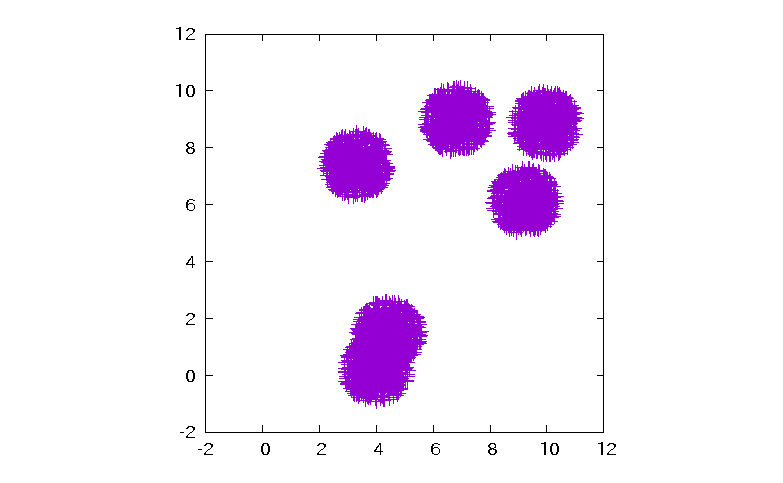
\includegraphics[height=.18\textheight]{fig/src2.eps}
 \end{center}
 \end{minipage}
 \begin{minipage}{.32\textwidth}
 \begin{center}
 \includegraphics[height=.18\textheight]{fig/src1.eps}
 \end{center}
 \end{minipage}
 \begin{minipage}{.32\textwidth}
 \begin{center}
 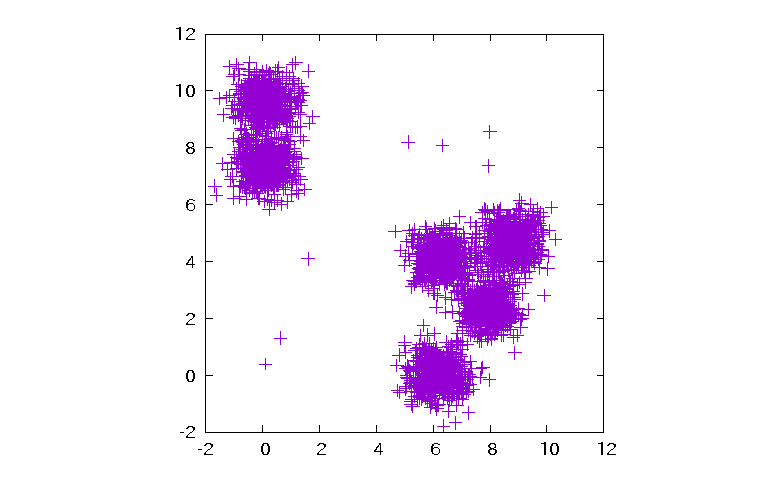
\includegraphics[height=.18\textheight]{fig/src3.eps}
 \end{center}
 \end{minipage}
\end{center}
\end{figure}
まず$K$-means法($K$-means++法)を試しました.
いずれの試行においても,同一の$K$に対し3回の結果を比較して最良のものを採用しました.
さらにシルエット分析に基づいて最適な$K$を選択しました.
\begin{figure}[h]
\begin{center}
 \begin{minipage}{.32\textwidth}
 \begin{center}
 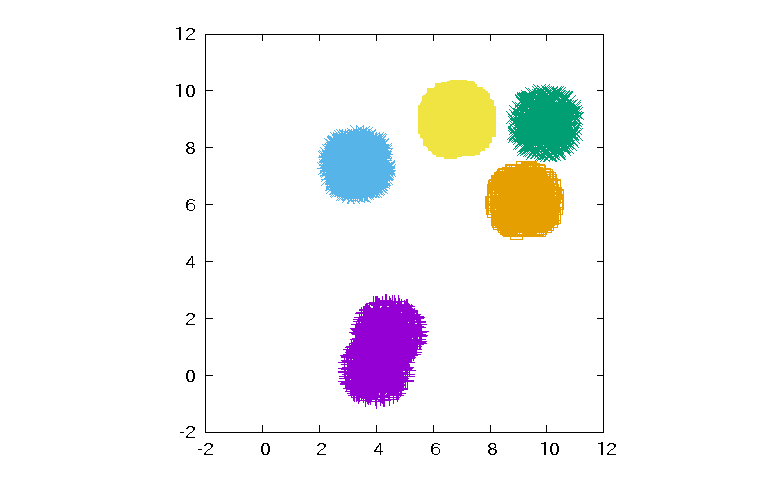
\includegraphics[height=.18\textheight]{fig/k2.eps}
 \end{center}
 \end{minipage}
 \begin{minipage}{.32\textwidth}
 \begin{center}
 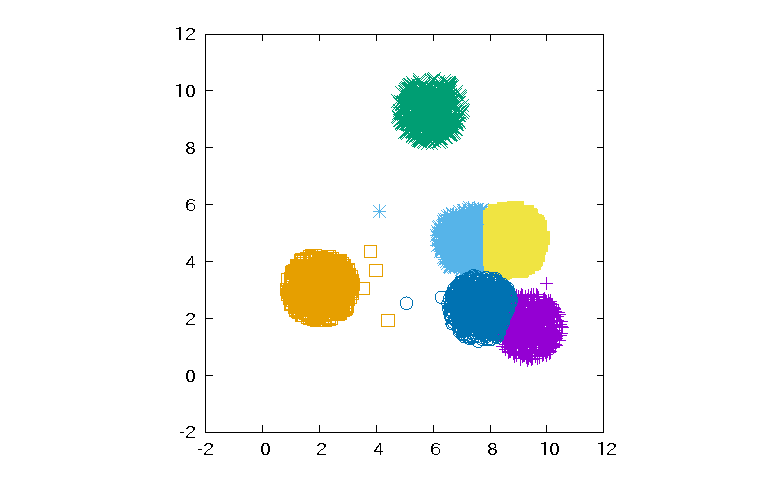
\includegraphics[height=.18\textheight]{fig/k1.eps}
 \end{center}
 \end{minipage}
 \begin{minipage}{.32\textwidth}
 \begin{center}
 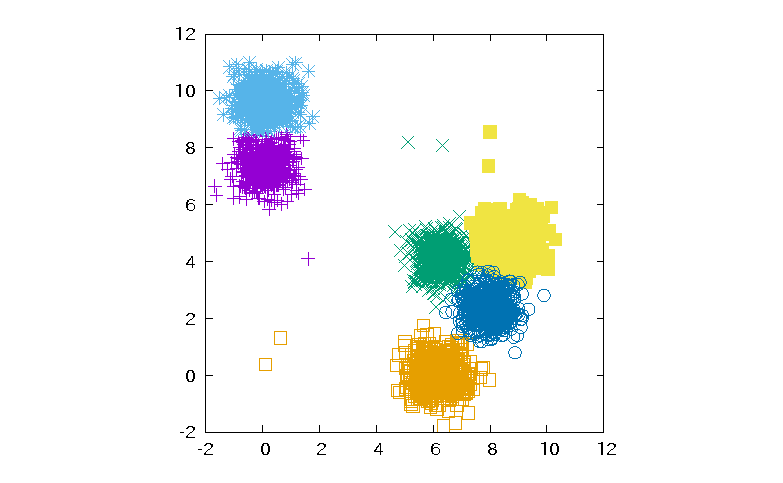
\includegraphics[height=.18\textheight]{fig/k3.eps}
 \end{center}
 \end{minipage}
\end{center}
\end{figure}
(A)のケースでは$K=5$,(B)(C)では$K=6$となりました.
それほど違和感の無い結果となっています.

次に$X$-meansを試しました.
\begin{figure}[h]
\begin{center}
 \begin{minipage}{.32\textwidth}
 \begin{center}
 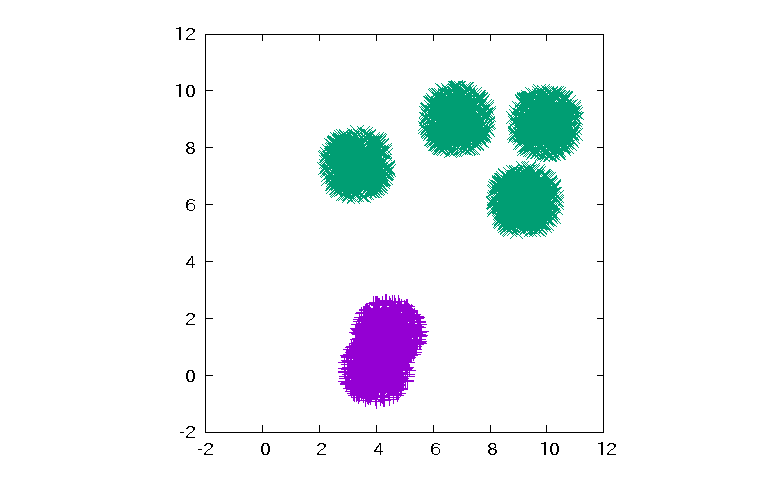
\includegraphics[height=.18\textheight]{fig/xb2.eps}
 \end{center}
 \end{minipage}
 \begin{minipage}{.32\textwidth}
 \begin{center}
 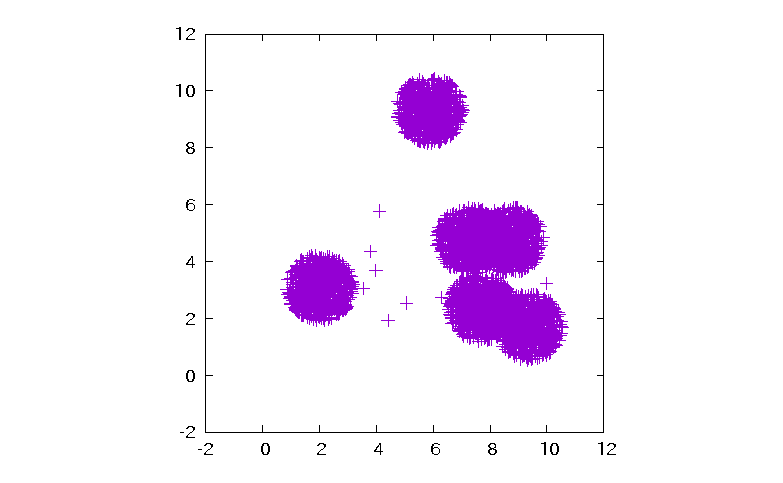
\includegraphics[height=.18\textheight]{fig/xb1.eps}
 \end{center}
 \end{minipage}
 \begin{minipage}{.32\textwidth}
 \begin{center}
 \includegraphics[height=.18\textheight]{fig/xb3.eps}
 \end{center}
 \end{minipage}
\end{center}
\end{figure}
(B)のケースではクラスタ分割が起こりませんでした.
(A)(C)も十分分割されているとは言えない結果になりました.

最後にEMアルゴリズムの結果です.
データセットに得られた確率密度関数を重ねて,立体的に可視化します.
\begin{figure}[h]
\begin{center}
 \begin{minipage}{.32\textwidth}
 \begin{center}
 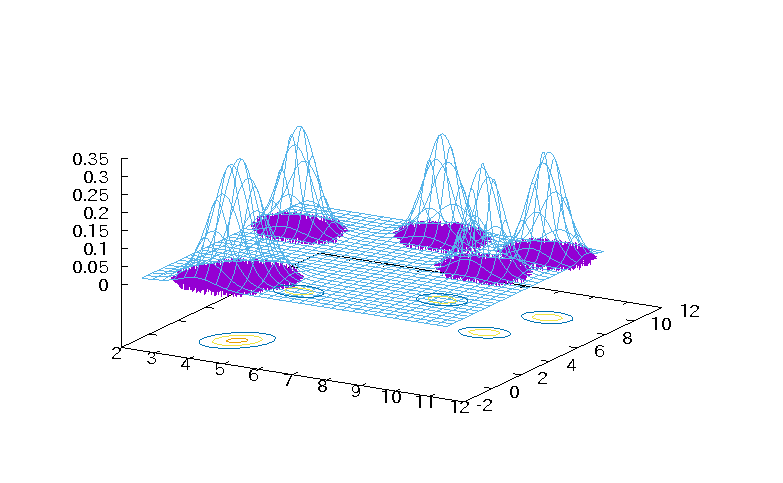
\includegraphics[height=.18\textheight]{fig/gmm2.eps}
 \end{center}
 \end{minipage}
 \begin{minipage}{.32\textwidth}
 \begin{center}
 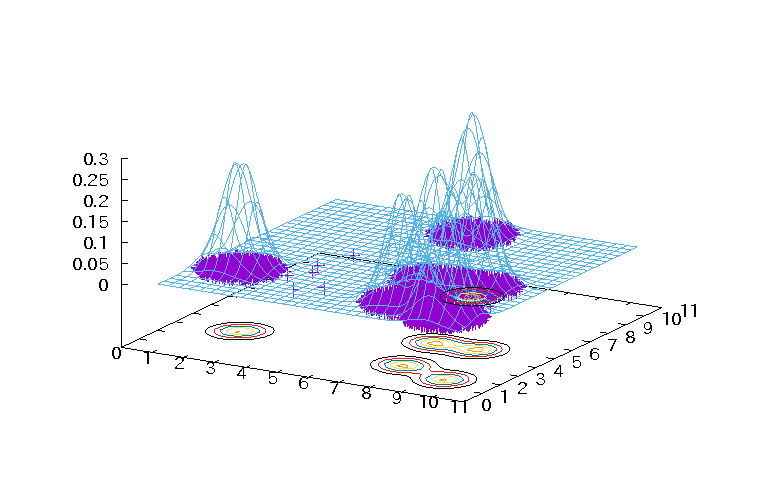
\includegraphics[height=.18\textheight]{fig/gmm1.eps}
 \end{center}
 \end{minipage}
 \begin{minipage}{.32\textwidth}
 \begin{center}
 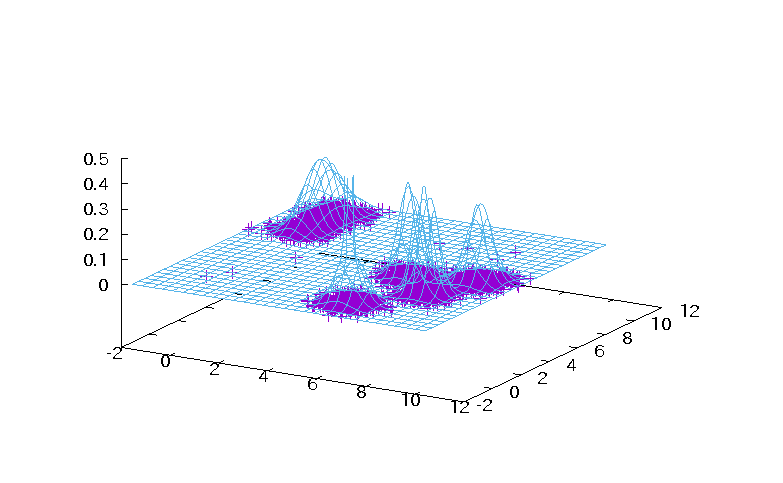
\includegraphics[height=.18\textheight]{fig/gmm3.eps}
 \end{center}
 \end{minipage}
\end{center}
\end{figure}
ただし$K$は全て6としています.
参考までに,$K$を$4\sim 9$と変えて得られたモデルのBICをプロットしたものが次のグラフです.
\begin{figure}[h]
\begin{center}
 \begin{minipage}{.32\textwidth}
 \begin{center}
 \includegraphics[height=.18\textheight]{fig/gmm2_bic.eps}
 \end{center}
 \end{minipage}
 \begin{minipage}{.32\textwidth}
 \begin{center}
 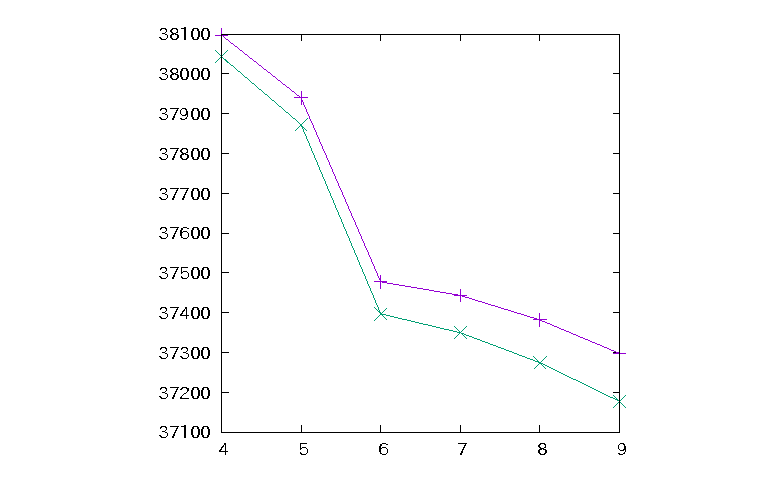
\includegraphics[height=.18\textheight]{fig/gmm1_bic.eps}
 \end{center}
 \end{minipage}
 \begin{minipage}{.32\textwidth}
 \begin{center}
 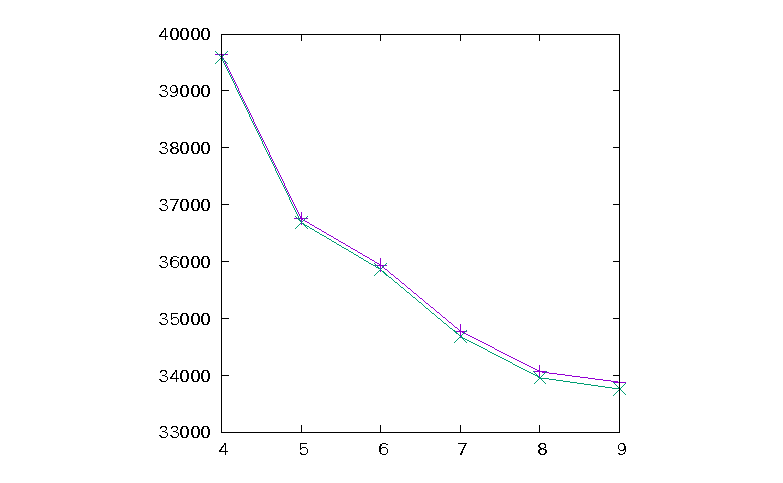
\includegraphics[height=.18\textheight]{fig/gmm3_bic.eps}
 \end{center}
 \end{minipage}
\end{center}
\end{figure}
紫線がBICです.
緑線はAIC(赤池情報量基準)\cite{bib:akaike1973}と呼ばれる別の指標です.
詳細は割愛します.
どちらの値も,(A)(B)のケースでは生成クラスタ数$K=6$に対し大きく低下しているものの,
最小値とはなっておらず,それより大きい$K$に対して減少していっています.
(C)のケースでは減少傾向にあまり特徴がありません.
いずれにしても,これを見て$K$を自動的に決定するのは難しそうです.

おまけで,
$\hat{\bm{f}}(\bm{x};\bm{\theta})=\bm{\theta}^{\mathrm{T}}\bm{x}-1$($k=1,2,3$,$n=3$)とし
$\bm{\theta}_{1}$,$\bm{\theta}_{2}$,$\bm{\theta}_{3}$を乱数的に作成したときの
$K$-means法およびEMアルゴリズムの結果を示します.
\begin{figure}[h]
\begin{center}
 \begin{minipage}{.4\textwidth}
 \begin{center}
 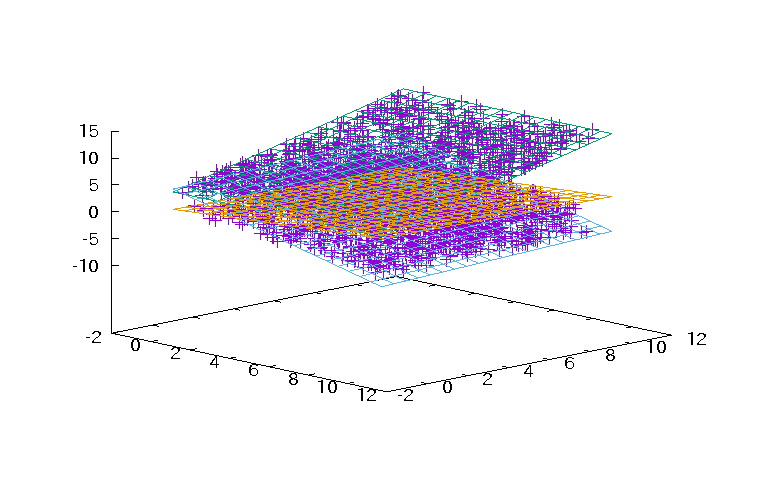
\includegraphics[height=.2\textheight]{fig/k_plane.eps}
 \end{center}
 \end{minipage}
 \begin{minipage}{.4\textwidth}
 \begin{center}
 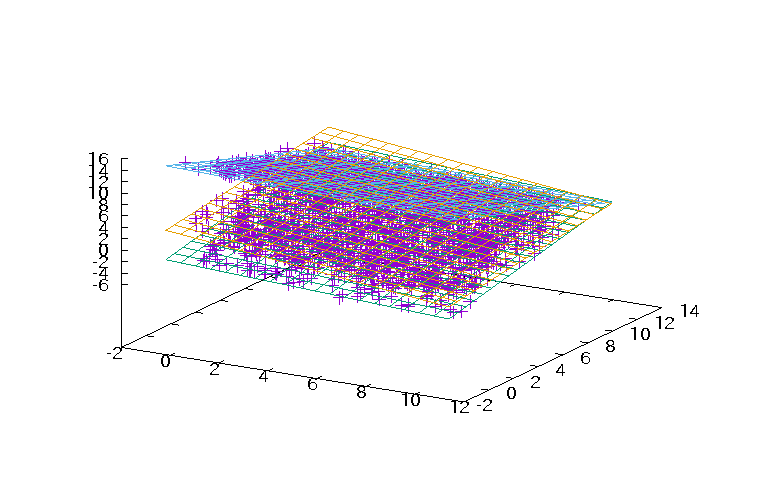
\includegraphics[height=.2\textheight]{fig/g_plane.eps}
 \end{center}
 \end{minipage}
\end{center}
\end{figure}
ちょっと分かりにくいですが,
どちらの方法でも平面をうまく推定できていることが見てとれるかと思います.

\section{まとめ}

複合代数的システムのモデル同定は典型的なchicken-and-egg問題であり,
標本の所属する部分システムの推定とモデルパラメータの同定を同時に行う必要があります.
これには$K$-means法とEMアルゴリズムが応用できます.

使用者観点での両者の違いは,標本をクラスタリングするかしないかです.
性能差は,本記事で示したような単純なケースでは大きく無さそうです.
部分システムの重複が大きかったり,アウトライアが多かったりするケースではEMアルゴリズムが有利になるだろうと予想は出来ますが,未検証です.

部分システム数$K$が未知の場合,
$K$-means法ならばシルエット分析によって自動推定することができます.
$X$-means法は残念ながら信頼できる方法では無さそうです.
EMアルゴリズムにおいては,
BICやAICは参考にはなるものの,直接的な自動推定の規範にはなりません.
他にうまい自動推定のやり方があるかどうかは十分調査できていません.



%%%%%%%%%%%%%%%%%%%%%%%%%%%%%%%%%%%%%%%%%%%%%%%%%%%%%%%%%%%%%%%%%%%%%%

\bibliographystyle{unsrt}
\begin{thebibliography}{99}
\bibitem{bib:macqueen1967}
J. B. MacQueen,
``Some Methods for Classification and Analysis of Multivariate Observations,''
in Proceedings of the fifth Berkeley Symposium on Mathematical Statistics and Probability 1, University of California Press, 1967.
\bibitem{bib:duda1973}
R. O. Duda and P. E. Hart,
``Pattern Classification and Scene Analysis,'' John Wiley {\&} Sons, 1973.
\bibitem{bib:katsavounidis1994}
I. Katsavounidis, C. C. J. Kuo and Z. Zhang,
``A New Initialization Technique for Generalized Lloyd Iteration,''
IEEE Signal Processing Letters, Vol. 1, No. 10, pp. 144--146, 1994.
\bibitem{bib:arthur2007}
D. Arthur and S. Vassilivitskii,
``k-means++: the advantages of careful seeding,''
in Proceedings of the 18th Annual ACM-SIAM Symposium on Discrete Algorithm, pp. 1027--1035, 2007.
\bibitem{bib:rousseeuw1987cam}
P. J. Rousseeuw,
``Silhouettes: a Graphical Aid to the Interpretation and Validation of Cluster Analysis,''
Computational and Applied Mathematics, Vol. 20, pp. 53--65, 1987.
\bibitem{bib:deAmorim2015is}
R. C. de Amorim and C. Hennig,
``Recovering the number of clusters in data sets with noise features using feature rescaling factors,''
Information Sciences, Vol. 324, pp. 126--145, 2015.
\bibitem{bib:pelleg2000}
D. Pelleg and A. Moore,
``$X$-means: Extending $K$-means with Efficient Estimation of the Number of Clusters,''
ICML-2000.
\bibitem{bib:shwarz1978}
G. Schwarz,
``Estimating the Dimension of a Model,''
Annual Statistics, Vol. 6, No. 2, pp.461--464, 1978.
\bibitem{bib:dempster1977}
A. P. Dempster, N. M. Laird, D. B. Rubin,
``Maximum Likelihood from Incomplete Data via the EM Algorithm,''
Journal of the Royal Statistical Society, Series B (Methodological), Vol. 39, No. 1, pp.1--38, 1977.
\bibitem{bib:akaike1973}
H. Akaike,
``Information theory and an extension of the maximum likelihood principle,''
in Proceedings of the 2nd International Symposium on Information Theory, Akadimiai Kiado, Budapest, pp. 267--281, 1973.
\end{thebibliography}



\end{document}
